\documentclass[11pt,oneside]{article}

\pdfminorversion=7
\usepackage{QuizStyle}

\hypersetup{
    pdftitle={20261111 Quiz for MATH200 Differential Equations},
    pdfauthor={Jungwoo Kim},
    pdfsubject={Quiz for MATH200 Differential Equations},
    pdfcreator={LaTeX}
}

\begin{document}

\quiztitle{20261111 Quiz}

% Boyce Section 6.3, Problem 1.
\begin{problem}{6.3.1}
Sketch the graph of the function
\[
    g(t)=u_2(t)+2u_3(t)-6u_4(t),
    \qquad t\geq0.
\]
\end{problem}

\begin{solution}
Here $u_c(t)=H(t-c)$ denotes the unit step function, with $H(0)=1$ as in the textbook. The value of $g$ changes at $t=2, 3, 4$, and
\[
    g(t)=
    \begin{cases}
        0, & 0\leq t<2,\\
        1, & 2\leq t<3,\\
        3, & 3\leq t<4,\\
        -3, & t\geq4.
    \end{cases}
\]
The filled and open circles indicate included and excluded endpoint values, respectively.
\begin{center}
\begin{tikzpicture}
\begin{axis}[
    width=0.76\textwidth,
    height=0.38\textwidth,
    axis lines=middle,
    xmin=0, xmax=5.5,
    ymin=-3.8, ymax=4.2,
    xlabel={$t$}, ylabel={$g(t)$},
    xtick={0,1,2,3,4,5},
    ytick={-3,0,1,3},
    tick label style={font=\small},
    label style={font=\small},
    clip=false
]
    \addplot[black,thick] coordinates {(0,0) (2,0)};
    \addplot[black,thick] coordinates {(2,1) (3,1)};
    \addplot[black,thick] coordinates {(3,3) (4,3)};
    \addplot[black,thick] coordinates {(4,-3) (5.35,-3)};
    \addplot[only marks,mark=o,mark size=2pt,black] coordinates {(2,0) (3,1) (4,3)};
    \addplot[only marks,mark=*,mark size=1.8pt,black] coordinates {(0,0) (2,1) (3,3) (4,-3)};
\end{axis}
\end{tikzpicture}
\end{center}
\end{solution}

% Boyce Section 6.3, Problem 2.
\begin{problem}{6.3.2}
Sketch the graph of the function
\[
    g(t)=f(t-\pi)u_\pi(t),
    \qquad f(t)=3t^2,
    \qquad t\geq0.
\]
\end{problem}

\begin{solution}
Because $u_\pi(t)=H(t-\pi)$, the function is
\[
    g(t)=
    \begin{cases}
        0, & 0\leq t<\pi,\\
        3(t-\pi)^2, & t\geq\pi.
    \end{cases}
\]
Thus the graph coincides with the $t$-axis until $t=\pi$ and then follows an upward-opening parabola with vertex $(\pi, 0)$.
\begin{center}
\begin{tikzpicture}
\begin{axis}[
    width=0.76\textwidth,
    height=0.38\textwidth,
    axis lines=middle,
    xmin=0, xmax=6.6,
    ymin=-1.2, ymax=35,
    xlabel={$t$}, ylabel={$g(t)$},
    xtick={0,3.14159265359,6.28318530718},
    xticklabels={$0$,$\pi$,$2\pi$},
    ytick={0,10,20,30},
    tick label style={font=\small},
    label style={font=\small},
    clip=false,
    samples=200
]
    \addplot[black,thick] coordinates {(0,0) (3.14159265359,0)};
    \addplot[black,thick,domain=3.14159265359:6.5] {3*(x-pi)^2};
    \addplot[only marks,mark=*,mark size=1.8pt,black] coordinates {(3.14159265359,0)};
\end{axis}
\end{tikzpicture}
\end{center}
\end{solution}

% Boyce Section 6.3, Problem 7 (both parts).
\begin{problem}{6.3.7}
Consider the function
\[
    f(t)=
    \begin{cases}
        t, & 0\leq t<1,\\
        t-1, & 1\leq t<2,\\
        t-2, & 2\leq t<3,\\
        0, & t\geq3.
    \end{cases}
\]
\begin{problemsubparts}
    \item Sketch the graph of $f$.
    \item Express $f(t)$ in terms of the unit step function $u_c(t)$.
\end{problemsubparts}
\end{problem}

\begin{solution}
\noindent\textup{(a)} On each of the intervals $[0, 1)$, $[1, 2)$, and $[2, 3)$, the graph is a line segment of slope $1$. The function jumps from the left-hand limit $1$ to $0$ at $t=1, 2, 3$.
\begin{center}
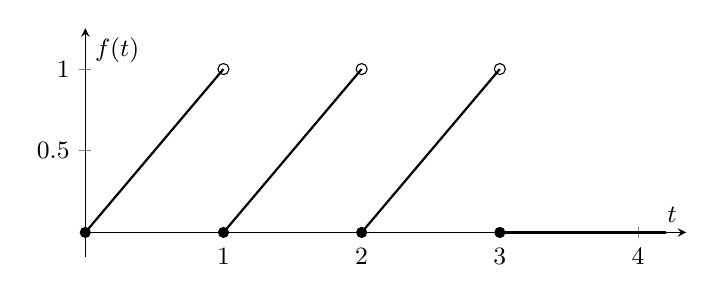
\begin{tikzpicture}
\begin{axis}[
    width=0.76\textwidth,
    height=0.37\textwidth,
    axis lines=middle,
    xmin=0, xmax=4.35,
    ymin=-0.15, ymax=1.25,
    xlabel={$t$}, ylabel={$f(t)$},
    xtick={0,1,2,3,4},
    ytick={0,0.5,1},
    tick label style={font=\small},
    label style={font=\small},
    clip=false
]
    \addplot[black,thick] coordinates {(0,0) (1,1)};
    \addplot[black,thick] coordinates {(1,0) (2,1)};
    \addplot[black,thick] coordinates {(2,0) (3,1)};
    \addplot[black,thick] coordinates {(3,0) (4.2,0)};
    \addplot[only marks,mark=o,mark size=2pt,black] coordinates {(1,1) (2,1) (3,1)};
    \addplot[only marks,mark=*,mark size=1.8pt,black] coordinates {(0,0) (1,0) (2,0) (3,0)};
\end{axis}
\end{tikzpicture}
\end{center}

\noindent\textup{(b)} Starting from $t$, subtract $1$ at both $t=1$ and $t=2$, and then subtract $t-2$ for $t\geq3$. Thus
\[
    \boxed{f(t)=t-u_1(t)-u_2(t)-(t-2)u_3(t)}.
\]
Equivalently, since $u_c(t)=H(t-c)$,
\[
    f(t)=t-H(t-1)-H(t-2)-(t-2)H(t-3).
\]
\end{solution}

% Boyce Section 6.3, Problem 9.
\begin{problem}{6.3.9}
Find the Laplace transform of
\[
    f(t)=
    \begin{cases}
        0, & t<2,\\
        (t-2)^3, & t\geq2.
    \end{cases}
\]
\end{problem}

\begin{solution}
Since $f(t)=H(t-2)(t-2)^3$, the second shifting theorem gives
\[
    \mathcal{L}\{f(t)\}(s)
    =e^{-2s}\mathcal{L}\{t^3\}(s)
    =e^{-2s}\frac{3!}{s^4}.
\]
Therefore
\[
    \boxed{\mathcal{L}\{f(t)\}(s)=\frac{6e^{-2s}}{s^4}}, \qquad s>0.
\]
\end{solution}

% Boyce Section 6.3, Problem 15.
\begin{problem}{6.3.15}
Find the inverse Laplace transform of
\[
    F(s)=\frac{(s-2)e^{-2s}}{s^2-4s+3}.
\]
\end{problem}

\begin{solution}
Complete the square in the denominator:
\[
    s^2-4s+3=(s-2)^2-1.
\]
Since
\[
    \mathcal{L}\{e^{2t}\cosh t\}(s)
    =\frac{s-2}{(s-2)^2-1},
\]
the factor $e^{-2s}$ produces a shift by $2$ in time. Therefore
\[
    \boxed{
        \mathcal{L}^{-1}\{F(s)\}(t)
        =H(t-2)e^{2(t-2)}\cosh(t-2)
    }.
\]
\end{solution}

% Boyce Section 6.3, Problem 21.
\begin{problem}{6.3.21}
Find the Laplace transform of the function
\[
    f(t)=
    \begin{cases}
        1, & 0\leq t<1,\\
        0, & 1\leq t<2,\\
        1, & 2\leq t<3,\\
        0, & t\geq3.
    \end{cases}
\]
\end{problem}

\begin{solution}
The function is nonzero only on $[0, 1)$ and $[2, 3)$. Hence
\[
    \begin{aligned}
    \mathcal{L}\{f(t)\}(s)
       &=\int_0^1 e^{-st}\,\dd t+\int_2^3 e^{-st}\,\dd t\\
       &=\frac{1-e^{-s}}{s}+\frac{e^{-2s}-e^{-3s}}{s}.
    \end{aligned}
\]
Thus
\[
    \boxed{\mathcal{L}\{f(t)\}(s)
    =\frac{1-e^{-s}+e^{-2s}-e^{-3s}}{s}},
    \qquad s>0.
\]
\end{solution}

% Boyce Section 6.4, Problem 2(a), (b), omitting (c), (d).
\begin{problem}{6.4.2}
Consider the initial value problem
\[
    y''+y=g(t), \qquad y(0)=0, \qquad y'(0)=2,
\]
where
\[
    g(t)=
    \begin{cases}
       t/2, & 0\leq t<6,\\
       3, & t\geq6.
    \end{cases}
\]
\begin{problemsubparts}
    \item Sketch the graph of the forcing function on an appropriate interval.
    \item Find the solution of the initial value problem.
\end{problemsubparts}
\end{problem}

\begin{solution}
\noindent\textup{(a)} The forcing function increases linearly from $g(0)=0$ to $g(6)=3$, and is constant thereafter. It is continuous at $t=6$.
\begin{center}
\begin{tikzpicture}
\begin{axis}[
    width=0.76\textwidth,
    height=0.37\textwidth,
    axis lines=middle,
    xmin=0, xmax=10.5,
    ymin=-0.25, ymax=4.2,
    xlabel={$t$}, ylabel={$g(t)$},
    xtick={0,3,6,9},
    ytick={0,1,2,3},
    tick label style={font=\small},
    label style={font=\small},
    clip=false
]
    \addplot[black,thick] coordinates {(0,0) (6,3)};
    \addplot[black,thick] coordinates {(6,3) (10.2,3)};
    \addplot[only marks,mark=*,mark size=1.8pt,black] coordinates {(0,0) (6,3)};
\end{axis}
\end{tikzpicture}
\end{center}

\noindent\textup{(b)} Since $g(t)=t/2$ for $t<6$ and then remains at $3$, it can be written as
\[
    g(t)=\frac{t}{2}-\frac{1}{2}H(t-6)(t-6).
\]
Taking Laplace transforms and using the initial conditions gives
\[
    (s^2+1)Y(s)-2
     =\frac{1-e^{-6s}}{2s^2},
\]
so
\[
    Y(s)=\frac{2}{s^2+1}
    +\frac{1-e^{-6s}}{2s^2(s^2+1)}.
\]
The partial fraction decomposition
\[
    \frac{1}{s^2(s^2+1)}=\frac{1}{s^2}-\frac{1}{s^2+1}
\]
shows that its inverse transform is $h(t)=t-\sin t$. Applying the second shifting theorem to the term containing $e^{-6s}$ yields
\[
    \boxed{
    y(t)=\frac32\sin t+\frac{t}{2}
    -\frac{1}{2}H(t-6)(t-6-\sin(t-6))
    }.
\]
For $0\leq t<6$, this gives $y''+y=t/2$. For $t>6$, the shifted term changes the forcing to $3$. The solution satisfies $y(0)=0$ and $y'(0)=2$, and both $y$ and $y'$ are continuous at $t=6$.
\end{solution}

% Boyce Section 6.5, Problem 2(a), presented as a standalone problem.
\begin{problem}{6.5.2}
Solve the initial value problem
\[
    y''-y=-5\delta(t-3), \qquad
    y(0)=1, \qquad y'(0)=0.
\]
\end{problem}

\begin{solution}
Taking Laplace transforms gives
\[
    (s^2-1)Y(s)-s=-5e^{-3s},
\]
so
\[
    Y(s)=\frac{s}{s^2-1}-\frac{5e^{-3s}}{s^2-1}.
\]
Using $\mathcal{L}^{-1}\{s/(s^2-1)\}(t)=\cosh t$ and $\mathcal{L}^{-1}\{1/(s^2-1)\}(t)=\sinh t$, we obtain
\[
    \boxed{y(t)=\cosh t-5H(t-3)\sinh(t-3)}.
\]
The impulse at $t=3$ leaves $y$ continuous and produces the jump $y'(3^+)-y'(3^-)=-5$, as required by the equation.
\end{solution}

% Boyce Section 6.6, Problem 4.
\begin{problem}{6.6.4}
Find the Laplace transform of
\[
    f(t)=\int_0^t(t-\tau)^2\cos(3\tau)\,\dd\tau.
\]
\end{problem}

\begin{solution}
With $p(t)=t^2$ and $q(t)=\cos(3t)$, the given function is $f=p\ast q$. By the convolution theorem,
\[
    \begin{aligned}
    \mathcal{L}\{f(t)\}(s)
      &=\mathcal{L}\{p(t)\}(s)\mathcal{L}\{q(t)\}(s)\\
      &=\frac{2}{s^3}\cdot\frac{s}{s^2+9}.
    \end{aligned}
\]
Therefore
\[
    \boxed{\mathcal{L}\{f(t)\}(s)=\frac{2}{s^2(s^2+9)}},
    \qquad s>0.
\]
\end{solution}

% Boyce Section 6.6, Problem 5.
\begin{problem}{6.6.5}
Find the Laplace transform of
\[
    f(t)=\int_0^t e^{-(t-\tau)}\sin(2\tau)\,\dd\tau.
\]
\end{problem}

\begin{solution}
Let $p(t)=e^{-t}$ and $q(t)=\sin(2t)$. Then $f=p\ast q$, so
\[
    \begin{aligned}
    \mathcal{L}\{f(t)\}(s)
       &=\mathcal{L}\{p(t)\}(s)\mathcal{L}\{q(t)\}(s)\\
       &=\frac{1}{s+1}\cdot\frac{2}{s^2+4}.
    \end{aligned}
\]
Hence
\[
    \boxed{\mathcal{L}\{f(t)\}(s)=\frac{2}{(s+1)(s^2+4)}},
    \qquad s>0.
\]
\end{solution}

% Boyce Section 6.6, Problem 6.
\begin{problem}{6.6.6}
Find the Laplace transform of
\[
    f(t)=\int_0^t\sin(t-\tau)\cos(2\tau)\,\dd\tau.
\]
\end{problem}

\begin{solution}
Here $p(t)=\sin t$ and $q(t)=\cos(2t)$, so $f=p\ast q$. Thus
\[
    \begin{aligned}
    \mathcal{L}\{f(t)\}(s)
       &=\mathcal{L}\{p(t)\}(s)\mathcal{L}\{q(t)\}(s)\\
       &=\frac{1}{s^2+1}\cdot\frac{s}{s^2+4}.
    \end{aligned}
\]
Therefore
\[
    \boxed{\mathcal{L}\{f(t)\}(s)=\frac{s}{(s^2+1)(s^2+4)}},
    \qquad s>0.
\]
\end{solution}

% Boyce Section 6.6, Problem 8.
\begin{problem}{6.6.8}
Find the inverse Laplace transform of
\[
    F(s)=\frac{1}{s^4(s^2+4)}
\]
by using the convolution theorem.
\end{problem}

\begin{solution}
Factor the transform as
\[
    F(s)=\frac{1}{s^4}\cdot\frac{1}{s^2+4}.
\]
The inverse transforms of the factors are
\[
    \mathcal{L}^{-1}\left\{\frac{1}{s^4}\right\}(t)=\frac{t^3}{6},
    \qquad
    \mathcal{L}^{-1}\left\{\frac{1}{s^2+4}\right\}(t)=\frac{1}{2}\sin(2t).
\]
By the convolution theorem,
\[
    \boxed{
       \mathcal{L}^{-1}\{F(s)\}(t)
       =\frac{1}{12}\int_0^t(t-\tau)^3\sin(2\tau)\,\dd\tau
    }.
\]
\end{solution}

% Boyce Section 6.6, Problem 9.
\begin{problem}{6.6.9}
Find the inverse Laplace transform of
\[
    F(s)=\frac{s}{(s+1)(s^2+9)}
\]
by using the convolution theorem.
\end{problem}

\begin{solution}
Write
\[
    F(s)=\frac{1}{s+1}\cdot\frac{s}{s^2+9}.
\]
The factors are the Laplace transforms of $e^{-t}$ and $\cos(3t)$, respectively. Hence
\[
    \boxed{
        \mathcal{L}^{-1}\{F(s)\}(t)
        =\int_0^t e^{-(t-\tau)}\cos(3\tau)\,\dd\tau
    }.
\]
\end{solution}

% Boyce Section 6.6, Problem 10.
\begin{problem}{6.6.10}
Find the inverse Laplace transform of
\[
    F(s)=\frac{1}{(s+1)^3(s^2+4)}
\]
by using the convolution theorem.
\end{problem}

\begin{solution}
We factor
\[
    F(s)=\frac{1}{(s+1)^3}\cdot\frac{1}{s^2+4},
\]
and use the inverse transforms
\[
    \mathcal{L}^{-1}\left\{\frac{1}{(s+1)^3}\right\}(t)
        =\frac{1}{2}t^2e^{-t},
    \qquad
    \mathcal{L}^{-1}\left\{\frac{1}{s^2+4}\right\}(t)
        =\frac{1}{2}\sin(2t).
\]
Thus
\[
    \boxed{
        \mathcal{L}^{-1}\{F(s)\}(t)
        =\frac{1}{4}\int_0^t(t-\tau)^2e^{-(t-\tau)}\sin(2\tau)\,\dd\tau
    }.
\]
\end{solution}

% Boyce Section 6.6, Problem 14.
\begin{problem}{6.6.14}
Express the solution of the initial value problem
\[
    4y''+4y'+17y=g(t),
    \qquad y(0)=0, \qquad y'(0)=1
\]
in terms of a convolution integral.
\end{problem}

\begin{solution}
Let $Y(s)=\mathcal{L}\{y(t)\}(s)$ and $G(s)=\mathcal{L}\{g(t)\}(s)$. The initial conditions yield
\[
    (4s^2+4s+17)Y(s)=G(s)+4.
\]
Since
\[
    4s^2+4s+17=4\left((s+\tfrac12)^2+4\right),
\]
we obtain
\[
    Y(s)=\frac{1}{(s+\tfrac12)^2+4}
    +\frac{G(s)}{4((s+\tfrac12)^2+4)}.
\]
The first term has inverse transform $\frac{1}{2}e^{-t/2}\sin(2t)$. The impulse-response kernel corresponding to the second term is
\[
    h(t)=\mathcal{L}^{-1}\left\{\frac{1}{4((s+\tfrac12)^2+4)}\right\}(t)
        =\frac{1}{8}e^{-t/2}\sin(2t).
\]
The convolution theorem now gives
\[
    \boxed{
        y(t)=\frac{1}{2}e^{-t/2}\sin(2t)
        +\frac{1}{8}\int_0^t e^{-(t-\tau)/2}\sin(2(t-\tau))g(\tau)\,\dd\tau
    }.
\]
\end{solution}

\end{document}
